% TEMPLATE for Usenix papers, specifically to meet requirements of
%  USENIX '05
% originally a template for producing IEEE-format articles using LaTeX.
%   written by Matthew Ward, CS Department, Worcester Polytechnic Institute.
% adapted by David Beazley for his excellent SWIG paper in Proceedings,
%   Tcl 96
% turned into a smartass generic template by De Clarke, with thanks to
%   both the above pioneers
% use at your own risk.  Complaints to /dev/null.
% make it two column with no page numbering, default is 10 point

% Munged by Fred Douglis <douglis@research.att.com> 10/97 to separate
% the .sty file from the LaTeX source template, so that people can
% more easily include the .sty file into an existing document.  Also
% changed to more closely follow the style guidelines as represented
% by the Word sample file. 

% Note that since 2010, USENIX does not require endnotes. If you want
% foot of page notes, don't include the endnotes package in the 
% usepackage command, below.

\documentclass[letterpaper,twocolumn,10pt]{article}
\usepackage{custom}
\usepackage{usenix,epsfig,endnotes,hyperref}
\usepackage{color, enumitem}
\usepackage{cleveref, float, graphicx, longtable, subcaption}

\begin{document}

%don't want date printed
\date{}

%make title bold and 14 pt font (Latex default is non-bold, 16 pt)
\title{\Large \bf Detection and Analysis of Disaster-Related Tweets}

\author{
{\rm Daniel Solomon}\\
\texttt{solomond@mail.tau.ac.il}
\and
{\rm Gal Ron}\\
\texttt{galr1@mail.tau.ac.il‬}
\and
{\rm Omri Ben-Horin}\\
\texttt{\red{EMAIL@mail.tau.ac.il}}
}

\maketitle

% Use the following at camera-ready time to suppress page numbers.
% Comment it out when you first submit the paper for review.
\thispagestyle{empty}


\abstract{}

\begin{center}
	\parbox{200pt}{
		\todo{bla bla bla bla bla bla bla bla bla bla bla bla bla bla bla bla bla bla bla bla bla bla bla bla bla bla bla bla bla bla bla bla bla bla bla bla bla bla bla bla bla bla bla bla bla bla bla bla bla bla bla bla bla bla bla bla bla bla bla bla bla bla bla bla bla bla bla bla bla bla bla bla bla bla bla bla bla bla bla bla bla bla bla bla bla bla bla bla bla bla bla bla bla bla bla bla bla bla bla bla bla bla bla bla bla bla bla bla.}
	}
\end{center}

%%%%%%%%%%%%%%%%%%%%%%%%%%%%%%%%%%%%%%%%%%
\section{Introduction}
The popular microblogging service Twitter is a fruitful source of user-created content. With hundreds of millions of new tweets every day, Twitter has become a probe to human behavior and opinions from around the globe. The Twitter 'corpus' reflects political and social trends, popular culture, global and local happenings, and more. In addition, tweets are easy to access and aggregate in real-time. Therefore, we experience an increased interest in natural language processing research of Twitter data.

As one of the world's most widely used social networks, Twitter is an effective channel of communication and plays an important role during a crisis or emergency. The live stream of tweets can be used to identify reports and calls for help in emergency situations, such as accidents, violent crimes, natural disasters and terror attacks (which we all refer to as 'disasters' in this paper).

In this work we utilize techniques from the natural language processing pipeline (tokenization, part-of-speech tagging and named-entity recognition) to work on Twitter data, as opposed to traditional corpora, in order to detect and analyze disaster-related tweets.

\paragraph{The Dataset}
We present our experiments on a \href{https://www.crowdflower.com/data-for-everyone/}{dataset} of 10,877 tweets\endnote{\textbf{"Disasters on social media" Dataset by CrowdFlower}: Contributors looked at over 10,000 tweets culled with a variety of searches like "ablaze", "quarantine", and "pandemonium", then noted whether the tweet referred to a disaster. \url{https://www.crowdflower.com/wp-content/uploads/2016/03/socialmedia-disaster-tweets-DFE.csv}}, labeled to \textit{'disaster-related'} and \textit{'not disaster-related'} with confidence in the range $[0,1]$. For example, the following tweet is \textit{'disaster-related'} with confidence 1,

\begin{center}
	\parbox{190pt}{\tweet{Thunderstorms with little rain expected in Central California. High fire danger. \#weather \#cawx http://t.co/A5GNzbuSqq}}
\end{center}


while the following tweet is \textit{'not disaster-related'} with confidence 0.59,

\begin{center}
	\parbox{190pt}{\tweet{It's been raining since you left me // Now I'm drowning in the flood // You see I've always been a fighter // But without you I give up}}
\end{center}

Even for one who is not familiar with the Bon Jovi lyrics in the latter tweet, it is clear that the tweet does not refer to a real natural disaster. However, this observation is hard to make examining only the vocabulary used; the latter tweet contains a variety of 'disastrous' words  (e.g. \tweet{raining, drowning, flood, fighter}). This example hints that in order to reach meaningful results we may have to examine additional linguistic features of colloquial writing,  as well as Twitter-specific features such as hashtags (\tweet{\textbf{\#}}), user at-mentions (\tweet{\textbf{@}}), internet links and emoticons.


\paragraph{Our Contribution}

In this paper we present our work tackling three missions involving disaster-related tweets.

The first mission is \textit{identification} of disaster-related tweets among a variety of tweets. We implemented several classifiers, the best of which achieved \todo{\%} accuracy on the dataset. We note that this method could have easily been adjusted to identify tweets related to themes other than disasters (e.g. politics-related, sports-related, etc.), given the appropriate dataset.

The second mission is binary classification of disaster-related tweets to one of two categories, \textit{subjective tweets} (i.e. tweets that express an emotion) vs. \textit{objective tweets} (such as news reports on disasters). To achieve this we manually tagged 2,410 disaster-related tweets. The motivation behind this task is that objective tweets like informative news reports are likely to be published after the event had already become clear to emergency services, while subjective tweets may contain invaluable first-person testimonies of ongoing events.

Finally, we extracted named entities to enrich our knowledge on the disaster (mostly location)... \todo{Omri - short description of method and achievements}.

To demonstrate our framework we aggregated recent tweets from various locations in the US, extracted disaster-related tweets using our classifier, and then used named-entity recognition to discover entities related to ongoing disasters. For example, "\tweet{Hurricane Harvey}" appeared as a top named-entity among recent tweets sent from Houston, TX, which we identified as \textit{disaster-related}.

The code of our project is available at \url{https://github.com/glrn/nlp-disaster-analysis}.

\subsection{Twitter vs. Traditional Corpora}

Tweets are limited to 140 characters and are widely used by non-professional writers. Therefore, Tweet datasets have some unique features that differ from traditional corpora (such as WSJ corpus). These features should be addressed when implementing natural language processing techniques.

First, the grammar of tweets is quite different from edited news text. It is common that tweets are written as colloquial sentences in first person where the subject ('I') is omitted, as in: '\tweet{see the flames from my window OMG}'.

Tweets are also characterized by extensive use of abbreviations and slang specific to social-media (e.g. \tweet{ily} for 'I love you', \tweet{iono} for 'I don't know). Such abbreviations may squash several parts-of-speech into one token, which poses a challenge to POS tagging. 

In addition, due to the colloquial nature of user-created content, it is common that proper words are replaced by phonetically or morphologically similar ones (e.g. 'wtchng' instead of 'watching', 'gr8' instead of 'great'). Users may also use capitalization irregularities, deliberate spelling errors, punctuation irregularities and interjections as a means to express their sentiment, as in the following tweet:

\begin{center}
	\parbox{190pt}{\tweet{Haha South Tampa is getting flooded hah- WAIT A SECOND I LIVE IN SOUTH TAMPA WHAT AM I GONNA DO WHAT AM I GONNA DO FVCK \#flooding}}
\end{center}

Lastly, tweets may contain a variety of tokens seen mainly in Twitter and other social media, such as: URLs; emoticons; Twitter hashtags, of the form \tweet{\#tagname}, which the authoer may supply to label a tweet; Twitter at-mentions of the form \tweet{@user} which link to other Twitter users; and Twitter discourse functions such as \tweet{RT} ("re-tweet"), indicating that a tweet was originally posted by some other Twitter user, or ellipsis dots (\tweet{...}) at the end (or beginning) of a tweet, indicating that the tweet will be continued in a subsequent tweet by the same user. We note that hashtags and at-mentions can also serve as words or phrases within a tweet, as in:

\begin{center}
	\parbox{190pt}{\tweet{Heard about the \#earthquake, stay safe everyone.}}
\end{center}

Regarding URLs, all links posted in tweets are shortened using Twitter's link service, \url{http://t.co}, and are converted to a seemingly random 23 characters URL that redirects to the original web address.
	

%%%%%%%%%%%%%%%%%%%%%%%%%%%%%%%%%%%%%%%%%%
\section{Analysis Wokrflow}

\paragraph{keywords} TODO

\begin{itemize}[noitemsep,nolistsep]
	\item A
	\item B
	\item C
\end{itemize}

\todo{(Gal) Complete this section}


%%%%%%%%%%%%%%%%%%%%%%%%%%%%%%%%%%%%%%%%%%
\section{Classification of Disaster-Related Tweets}

In the first part of our work we developed a classifier that identifies \textit{disaster-related} tweets from \textit{not disaster-related} tweets, trained on a dataset of 10,877 labeled tweets (\todo{note: maybe better to say that the dataset was ~2400 tweets, since we looked only at tweets with confident $>0.9$}) [\todo{Gal: Notice that using 0.9+ confidence filtered around 5000 tweets I think, 2400 were positive...}]. We experimented with a Naive Bayes (NB), random forest (RF) and support vector machine (SVM) classifiers.

\paragraph{Naive Bayes}
A supervised probabilistic learning method that classify according to \textit{maximum a posteriori}. In this method we used \textit{unigram} and \textit{bigram} features.

\paragraph{Random Forest}
An ensemble learning method that uses some estimators (trees) to classify. In this method we used \textit{unigram} and \textit{bigram} features.

\paragraph{Support Vector Machine (SVM)}
A discriminative learning method that attempts to find the hyperplane that gives maximum margin between positive and negative classification on the training data, using penalty method for mistakes. In this method we used \textit{unigram}, \textit{bigram}, \textit{tweets metadata} and \textit{POS tagging} features.
 
\subsection{Feature Extraction}

To train the classifiers we extracted several features for each tweet:

\begin{itemize}[noitemsep]
	\item \textbf{Unigrams and bigrams} of tokens in tweet; we used a Python version of \texttt{Twokenizer}, tokenizer for Twitter data (Gimpel et al. \cite{POS-Tagging}, Myle Ott, 2013 \cite{ark-twokenize-py}).
	\item \textbf{Tweet metadata}; hashtags, at-mentions and URLs; we parsed the tweet, crawled URLs and used the referred webpage title as supplementary information.
	\item \textbf{Part-of-speech (POS) tags} (bigram and unigram); we used a twitter-specific tagset and tagger presented by Gimpel et al. \cite{POS-Tagging}.
\end{itemize}

\paragraph{Tokenization}
Splitting a tweet to tokens (separated ordered words) is hard due to irregular punctuation patterns and use of punctuation marks for emoticons. For example, the correct tokenization of '\tweet{hello (\#hashtag)}' is to the four tokens [\tweet{ hello , ( , \#hashtag , ) }], but '\tweet{hello (:}' should be split only to the tuple [ \tweet{hello , (:} ].

\texttt{Twokenizer} is a tokenizer designed for Twitter text in English that addresses these issues. It was originally developed in Python by O'Connor et al., 2010 \cite{TweetMotif}, then improved and ported to Java by Gimpel et al., 2011 \cite{POS-Tagging} and later ported back to Python \cite{ark-twokenize-py}. We use the last version by Myle Ott.

\paragraph{Metadata Extraction}
The hashtags, at-mentions, URLs and emoticons in a tweet carry information that may help better understand the subject and context. Therefore, for each tweet we created a vector of the following metadata features, which we found to be the most expressive:

\begin{itemize}[noitemsep, nolistsep]
	\item Does the tweet contain a link?
	\item How many link are in tweet?
	\item Is '\texttt{https://twitter.com}' one of the links?
	\item Does the tweet contain a user at-mention?
	\item Does the tweet contain a hashtag?
	\item How many hashtags are in tweet?
	\item Does the tweet contain a happy emoticon?
\end{itemize}

In addition to these features, we extracted information from hashtags and URLs. We attempted to split hashtgs to separate words 
looking for a CamelCase pattern (for example, \tweet{\#JeSuisCharlie} $\rightarrow$ 'Je Suis Charlie') or words separated by underline. We note that this method is not exhaustive since Twitter users tend to create hashtags composed of joined words, all lower-case.

We also found that the domain name of the URLs in a tweet may give an indication to whether the tweet is disaster-related or not (for example, a link to \texttt{https://9gag.com} is a negative hint). However, Twitter applies URL shortening on links, so for each shortened link in the dataset we attempted to reach the original Internet address. We also collected the HTML page title, which often contains the title of an article (for example, in news sites). We managed to expand 4,823 URLs out of 6,157 in the dataset.

For each tweet in the dataset we created an 'extended' version with extracted hashtag, expanded URL, and where every user at-mention is replaced by the token \_\_USERREF\_\_. For example, the following is a tweet,

\begin{center}
	\parbox{190pt}{\todo{\tweet{Gal}}}
\end{center}

and its extended version is,

\begin{center}
	\parbox{190pt}{\todo{\tweet{Gal}}}
\end{center}

\paragraph{Twitter POS Tagging}
\todo{Gal \cite{POS-Tagging}}

\subsection{Results}
Dataset was divided into train (90\%) and test (10\%) sets. Each classification method was tested with \textit{unigram} features and \textit{bigram} features separately, for the \textit{SVM} classifier, \textit{tweets metadata} and \textit{POS tagging} features were tested as well. \\
Accuracy was calculated by 3 measures:
\paragraph{Total Accuracy} number of right classifications out of the total queries ($ \frac{TP + TN}{TP + FP + TN + FN } $).
\paragraph{Positive Predictive Value} number of right positive classifications out of total positive classifications ($ \frac{TP}{TP + FP} $).
\paragraph{Negative Predictive Value} number of right negative classifications out of total negative classifications ($ \frac{TN}{TN + FN} $).
\\\\
For both \textit{Random Forest} and \textit{SVM} classifiers we have tuned parameters using \textit{grid search}. For \textit{Random Forest} we have tuned the number of estimators and for \textit{SVM} we have tuned the penalty constant. \\
\paragraph{Random Forest} For the \textit{Random Forest} results \ref{fig:disaster_classification_rf}, we can observe easily that the \textit{Unigram} features have better accuracy and better \textit{NPV}, while \textit{Bigram} features have better \textit{PPV} for any number of estimators. In addition, best result for total accuracy, \textit{PPV}, \textit{NPV} are achieved with 128, 64 and 128 estimators respectively.

\paragraph{SVM} For the \textit{SVM} results \ref{fig:disaster_classification_svm_uni} \ref{fig:disaster_classification_svm_bi}, we see that for \textit{Unigram} features with or without \textit{POS}, all measurements are becoming constant for $ C \ge 10^4 $ (penalty is too big to be used). In addition, best result for total accuracy, \textit{PPV}, \textit{NPV} are achieved penalty constant of value $ 10^4 $, $ 10^3 $  and $ 10^4 $ respectively. For \textit{Bigram} features results are very familiar except for a minor gap (around 1.5\%) between using \textit{POS} and not. Best result for total accuracy, \textit{PPV}, \textit{NPV} are exactly the same as in the \textit{Unigram} features. Notice that all classifiers used \textit{tweets metadata} features as well.

The following tables \ref{tab:disaster_classifiaction_best_results_nb_and_rf}  \ref{tab:disaster_classifiaction_best_results_svm} presents the best measurement result for each classifier, best total accuracy results (94.5\%) are achieved with \textit{SVM} classifier using \textit{Bigram}, \textit{tweets metada} and \textit{POS-tagging} features. \\
As it can be seen, we have succeeded in classifying disaster related or not tweets with several very accurate techniques. \\
It is important to mention that although the accuracies are very high using simple methods, before preprocessing the tweets, partial measurements were taken and all accuracies were around 82\%, therefore preprocessing the tweets was a major improvement for the classification (over 10\%).

\begin{table}[H]
	\caption{Disaster Classification Best Results: Naive Bayes and Random Forest}
	\label{tab:disaster_classifiaction_best_results_nb_and_rf}
	\begin{center}
		\scalebox{0.8}{
			\begin{tabular}{c | c | c | c | c}
				  & $ \textbf{Uni NB} $ & $ \textbf{Bi NB} $ & $ \textbf{Uni RF} $ & $ \textbf{Bi RF} $ \\ \hline
				accuracy & 0.921 & 0.864 & 0.911 & 0.890  \\
				ppv & 0.977 & 1.000 & 0.945 & 0.969 \\
				npv & 0.891 & 0.813 & 0.892 & 0.856 \\
			\end{tabular}
		}	
	\end{center}
\end{table}

\begin{table}[H]
	\caption{Disaster Classification Best Results: SVM}
	\label{tab:disaster_classifiaction_best_results_svm}
	\begin{center}
		\scalebox{0.8}{
			\begin{tabular}{c | c | c | c | c }
				 & $ \textbf{Uni SVM} $ & $ \textbf{Uni POS SVM} $ & $ \textbf{Bi SVM} $ & $ \textbf{Bi POS SVM} $ \\ \hline
				accuracy & 0.935 & 0.937 & 0.933 & 0.945 \\
				ppv & 0.961 & 0.946 & 0.952 & 0.955 \\
				npv & 0.935 & 0.938 & 0.926 & 0.939 \\
			\end{tabular}
		}	
	\end{center}
\end{table}

\begin{figure}[H]
	\centering
	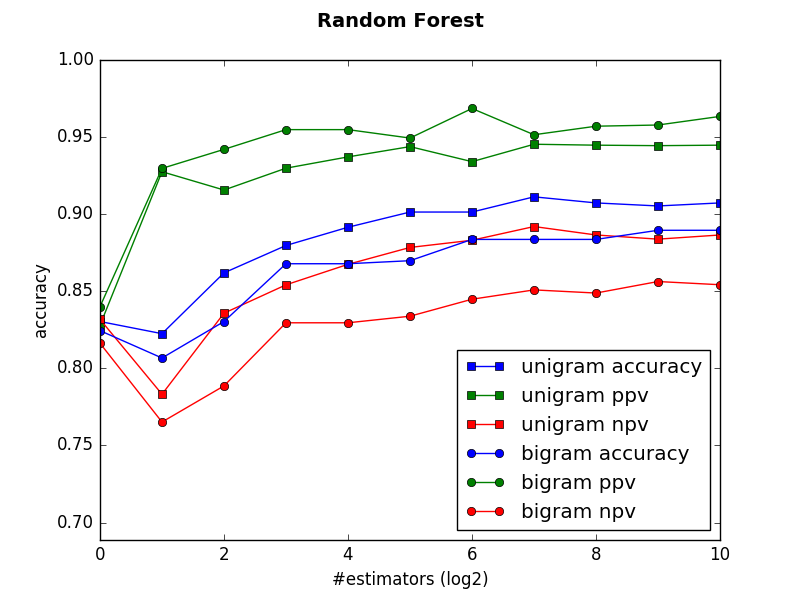
\includegraphics[width=\columnwidth]{../graphs/DisasterClassification/random_forest_unigram_vs_bigram_features.png}			
	\caption{Disaster Classification Random Forest (Unigram vs. Bigram)}
	\label{fig:disaster_classification_rf}
\end{figure}

\begin{figure}[H]
	\centering
	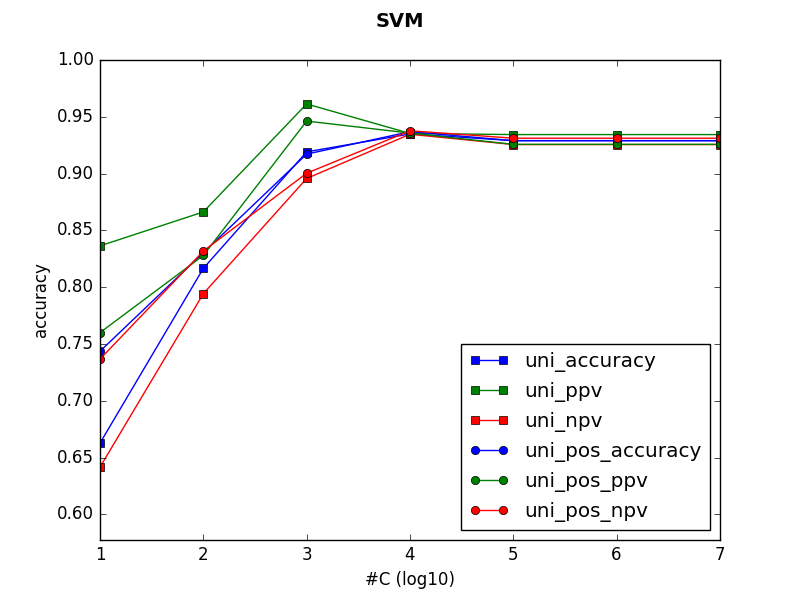
\includegraphics[width=\columnwidth]{../graphs/DisasterClassification/svm_uni_features.png}
	\caption{Disaster Classification SVM (Unigram vs. Unigram and POS)}
	\label{fig:disaster_classification_svm_uni}
\end{figure}
	
\begin{figure}[H]
	\centering
	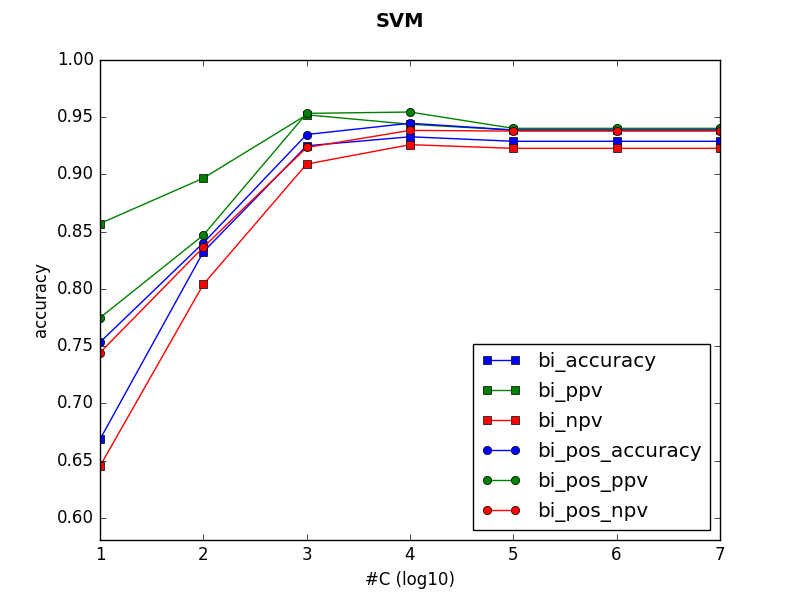
\includegraphics[width=\columnwidth]{../graphs/DisasterClassification/svm_bi_features.png}
	\caption{Disaster Classification SVM (Bigram vs. Bigram and POS)}
	\label{fig:disaster_classification_svm_bi}
\end{figure}		
	
%%%%%%%%%%%%%%%%%%%%%%%%%%%%%%%%%%%%%%%%%%
\section{Sentiment Analysis of Tweets}

\todo{}

%%%%%%%%%%%%%%%%%%%%%%%%%%%%%%%%%%%%%%%%%%
\section{Named-Entity Recognition in Tweets}

\todo{}

%%%%%%%%%%%%%%%%%%%%%%%%%%%%%%%%%%%%%%%%%%
\section{Experimenting with Recent Tweets}

\todo{(Gal) Complete this section}
\paragraph{keywords}Twitter's Search API


%%%%%%%%%%%%%%%%%%%%%%%%%%%%%%%%%%%%%%%%%%
\section{Conclusions}

\paragraph{Future work} TODO

%%%%%%%%%%%%%%%%%%%%%%%%%%%%%%%%%%%%%%%%%%

{\footnotesize \bibliographystyle{acm}
\bibliography{references}}

\theendnotes

\end{document}







